% \documentclass{article}
\documentclass[tikz,border=10pt]{standalone}
\usepackage[dvipsnames]{xcolor}
\usepackage{tikz}

\usetikzlibrary{backgrounds}
\usetikzlibrary{calc}
\usetikzlibrary{fit}
\usetikzlibrary{positioning}
\usetikzlibrary{math}
\usetikzlibrary{trees}
\begin{document}

% Define a macro to encapsulate rectangle logic with offsets
\newcommand{\drawgrouprect}[2]{%
    \draw[grouprect] 
        ($(#1.north west)+(-0.3,0.3)$) rectangle ($(#2.south east)+(0.3,-0.3)$);
}

% Define a reusable style for rectangles
\tikzset{
    grouprect/.style={
        draw=blue, % Rectangle border color
        thick, % Rectangle border thickness
        rounded corners=5pt, % Rounded corners with radius
    }
}

    % every node/.style={circle, draw},
    % level 1/.style={sibling distance=40mm, level distance=15mm},
    % level 2/.style={sibling distance=10mm, level distance=15mm},
    % edge from parent/.style={draw, -stealth}
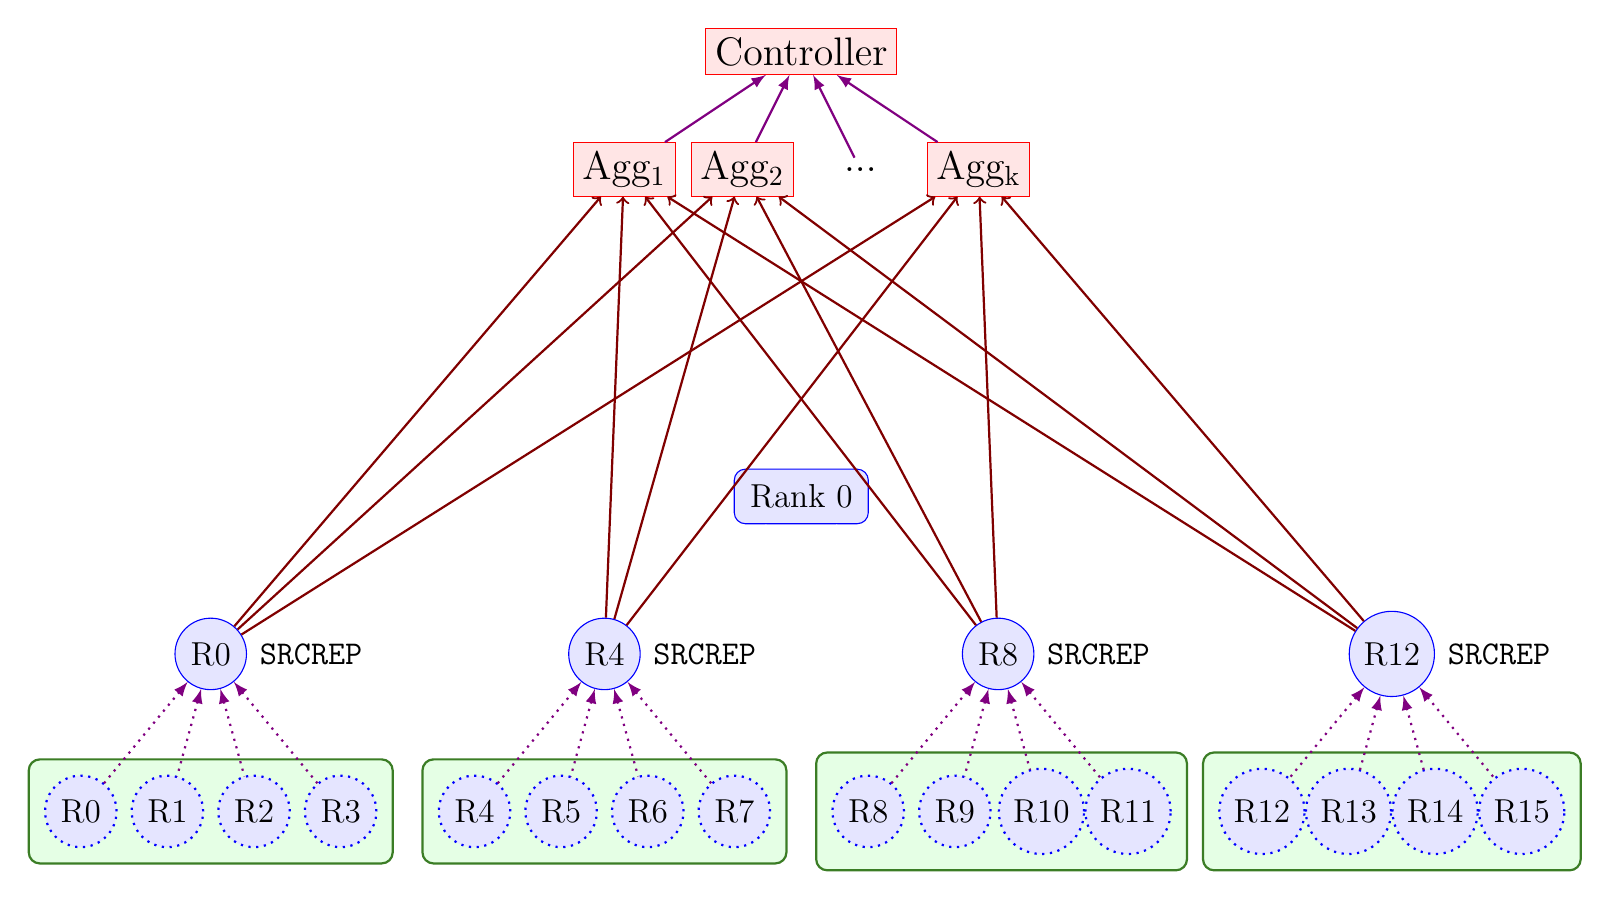
\begin{tikzpicture}[
  % level distance=4cm, sibling distance=4cm
  % grow via three points={
  %   one child at (0,-1) and two children at (-.5,-1) and (.5,-1)
  % },
  % level 1/.style={level distance=2cm,sibling distance=4cm},
  % level 2/.style={level distance=2cm,sibling distance=1cm}
  % level 3/.style={level distance=8cm,sibling distance=2cm}
  % every node/.style={font=\Huge, circle, draw=blue, fill=blue!20, minimum size=8mm},
  treeMon/.style={},
  % treeApp/.style={},
  % % level distance=4cm,sibling distance=5cm,
    % treeApp/.style={circle, draw=blue, fill=blue!20, minimum size=8mm},
]

\tikzset{
  nodeRanksRect/.style 2 args={
    draw=OliveGreen, thick, rounded corners,
    rectangle,
    fit={(#1) (#2)},
    inner sep=0.2cm,
    fill=green!10,
    on background layer
  }
}

\begin{scope}[
  every node/.style={font=\Large, rectangle, draw=red, fill=red!10, minimum size=2mm,align=center},
  edge from parent/.style={draw=Purple,thick,latex-}
  ]
\node [treeMon] (monRoot) {Controller}
child [treeMon]{node {Agg\textsubscript{1}}}
child [treeMon]{node {Agg\textsubscript{2}}}
child {node[draw=none, fill=none] {...}}
child [treeMon]{node {Agg\textsubscript{k}}}
;

\end{scope}

% --- Begin App Tree ---

\begin{scope}[
  level 1/.style={level distance=2cm,sibling distance=5cm},
  level 2/.style={level distance=2cm,sibling distance=1.1cm,
  edge from parent/.style={draw=Purple,thick,latex-,dotted}
  },
  every node/.style={font=\large,circle, draw=blue, fill=blue!10, minimum size=2mm,align=center},
  edge from parent/.style={draw=white,thick,latex-,dotted}
  ]
\node [inner sep=0.2cm,shape=rectangle,rounded corners,below=5cm of monRoot] (appRoot) {Rank 0}
child foreach \idx in {0,4,8,12} {
  node [label=0:\texttt{SRCREP}] {R\idx}
  child foreach \subidx in {0,1,2,3} {
    node {
      \tikzmath {
        integer \a, \b, \c;
        \a = \idx;
        \b = \subidx;
        \c = \idx + \subidx;
      }%
      R\c
    }
  }
};
\end{scope}

\begin{pgfonlayer}{background}
\node[nodeRanksRect={appRoot-1-1}{appRoot-1-4}] {};
\node[nodeRanksRect={appRoot-2-1}{appRoot-2-4}] {};
\node[nodeRanksRect={appRoot-3-1}{appRoot-3-4}] {};
\node[nodeRanksRect={appRoot-4-1}{appRoot-4-4}] {};
\end{pgfonlayer}

\foreach \x in {1,...,4} {
  \foreach \y in {1,2,4} {
    \draw[->,thick,color=Maroon] (appRoot-\x) -- (monRoot-\y);
  }
}

% \draw[->,thick,dotted,color=Purple] (monRoot) -- (appRoot);

\end{tikzpicture}
\end{document}
